\section{Results}

\subsection{Hardware design}

%As mentioned in the introduction, the team has to design and test hardware within a very short time.

%By reusing software and hardware design from last year's design, issues were reduced to a minimum.

The electronic design automation \emph{(EDA)} software used for schematics and pcb layout, \emph{Altium Nexus} supports multiple features which shortened the design process significantly. Firstly, since VCU19 used \emph{hierarchical design} (i.e. project is composed of multiple sheets and sub sheets), large parts of the schematics developed during last years design period could be reused. 

Simple sub circuits like CAN-FD transceivers could be directly copied without issue. In addition, the sub sheets are modular in the sense that they appear as an electrical component with a specific set of interfaces, or \emph{ports}. This means that sheet using the same set of ports can be interchanged freely. The modularity of the sheets was heavily used during the development of VCU20. The new processing unit features a super set of the VCU19 SoC interface, meaning they are perfectly compatible. 

There is also the possibility of reusing sheets in the same project. VCU20 has 4 CAN-FD transceivers, but since the transceiver schematic is identical for all 4 interfaces, the sheet can simply be repeated. 

There are also features for reuse in the PCB layout part of the design. Altium Nexus has a feature called \emph{rooms} which is a grouping of component footprints and how they are connected. It is possible to copy the layout if a room to other rooms. The designer chooses how rooms are generated, and by default they are created per sheet. This means that the layout for one CAN-FD transceiver can be perfected and then copied over to the other 3 transceiver rooms.

The PCB was produced by Simpro AS as they are sponsoring Revolve NTNU. The finished, soldered PCB can be seen in figure \ref{fig:vcu20_soldered}.

\begin{figure}[h!]
    \centering
    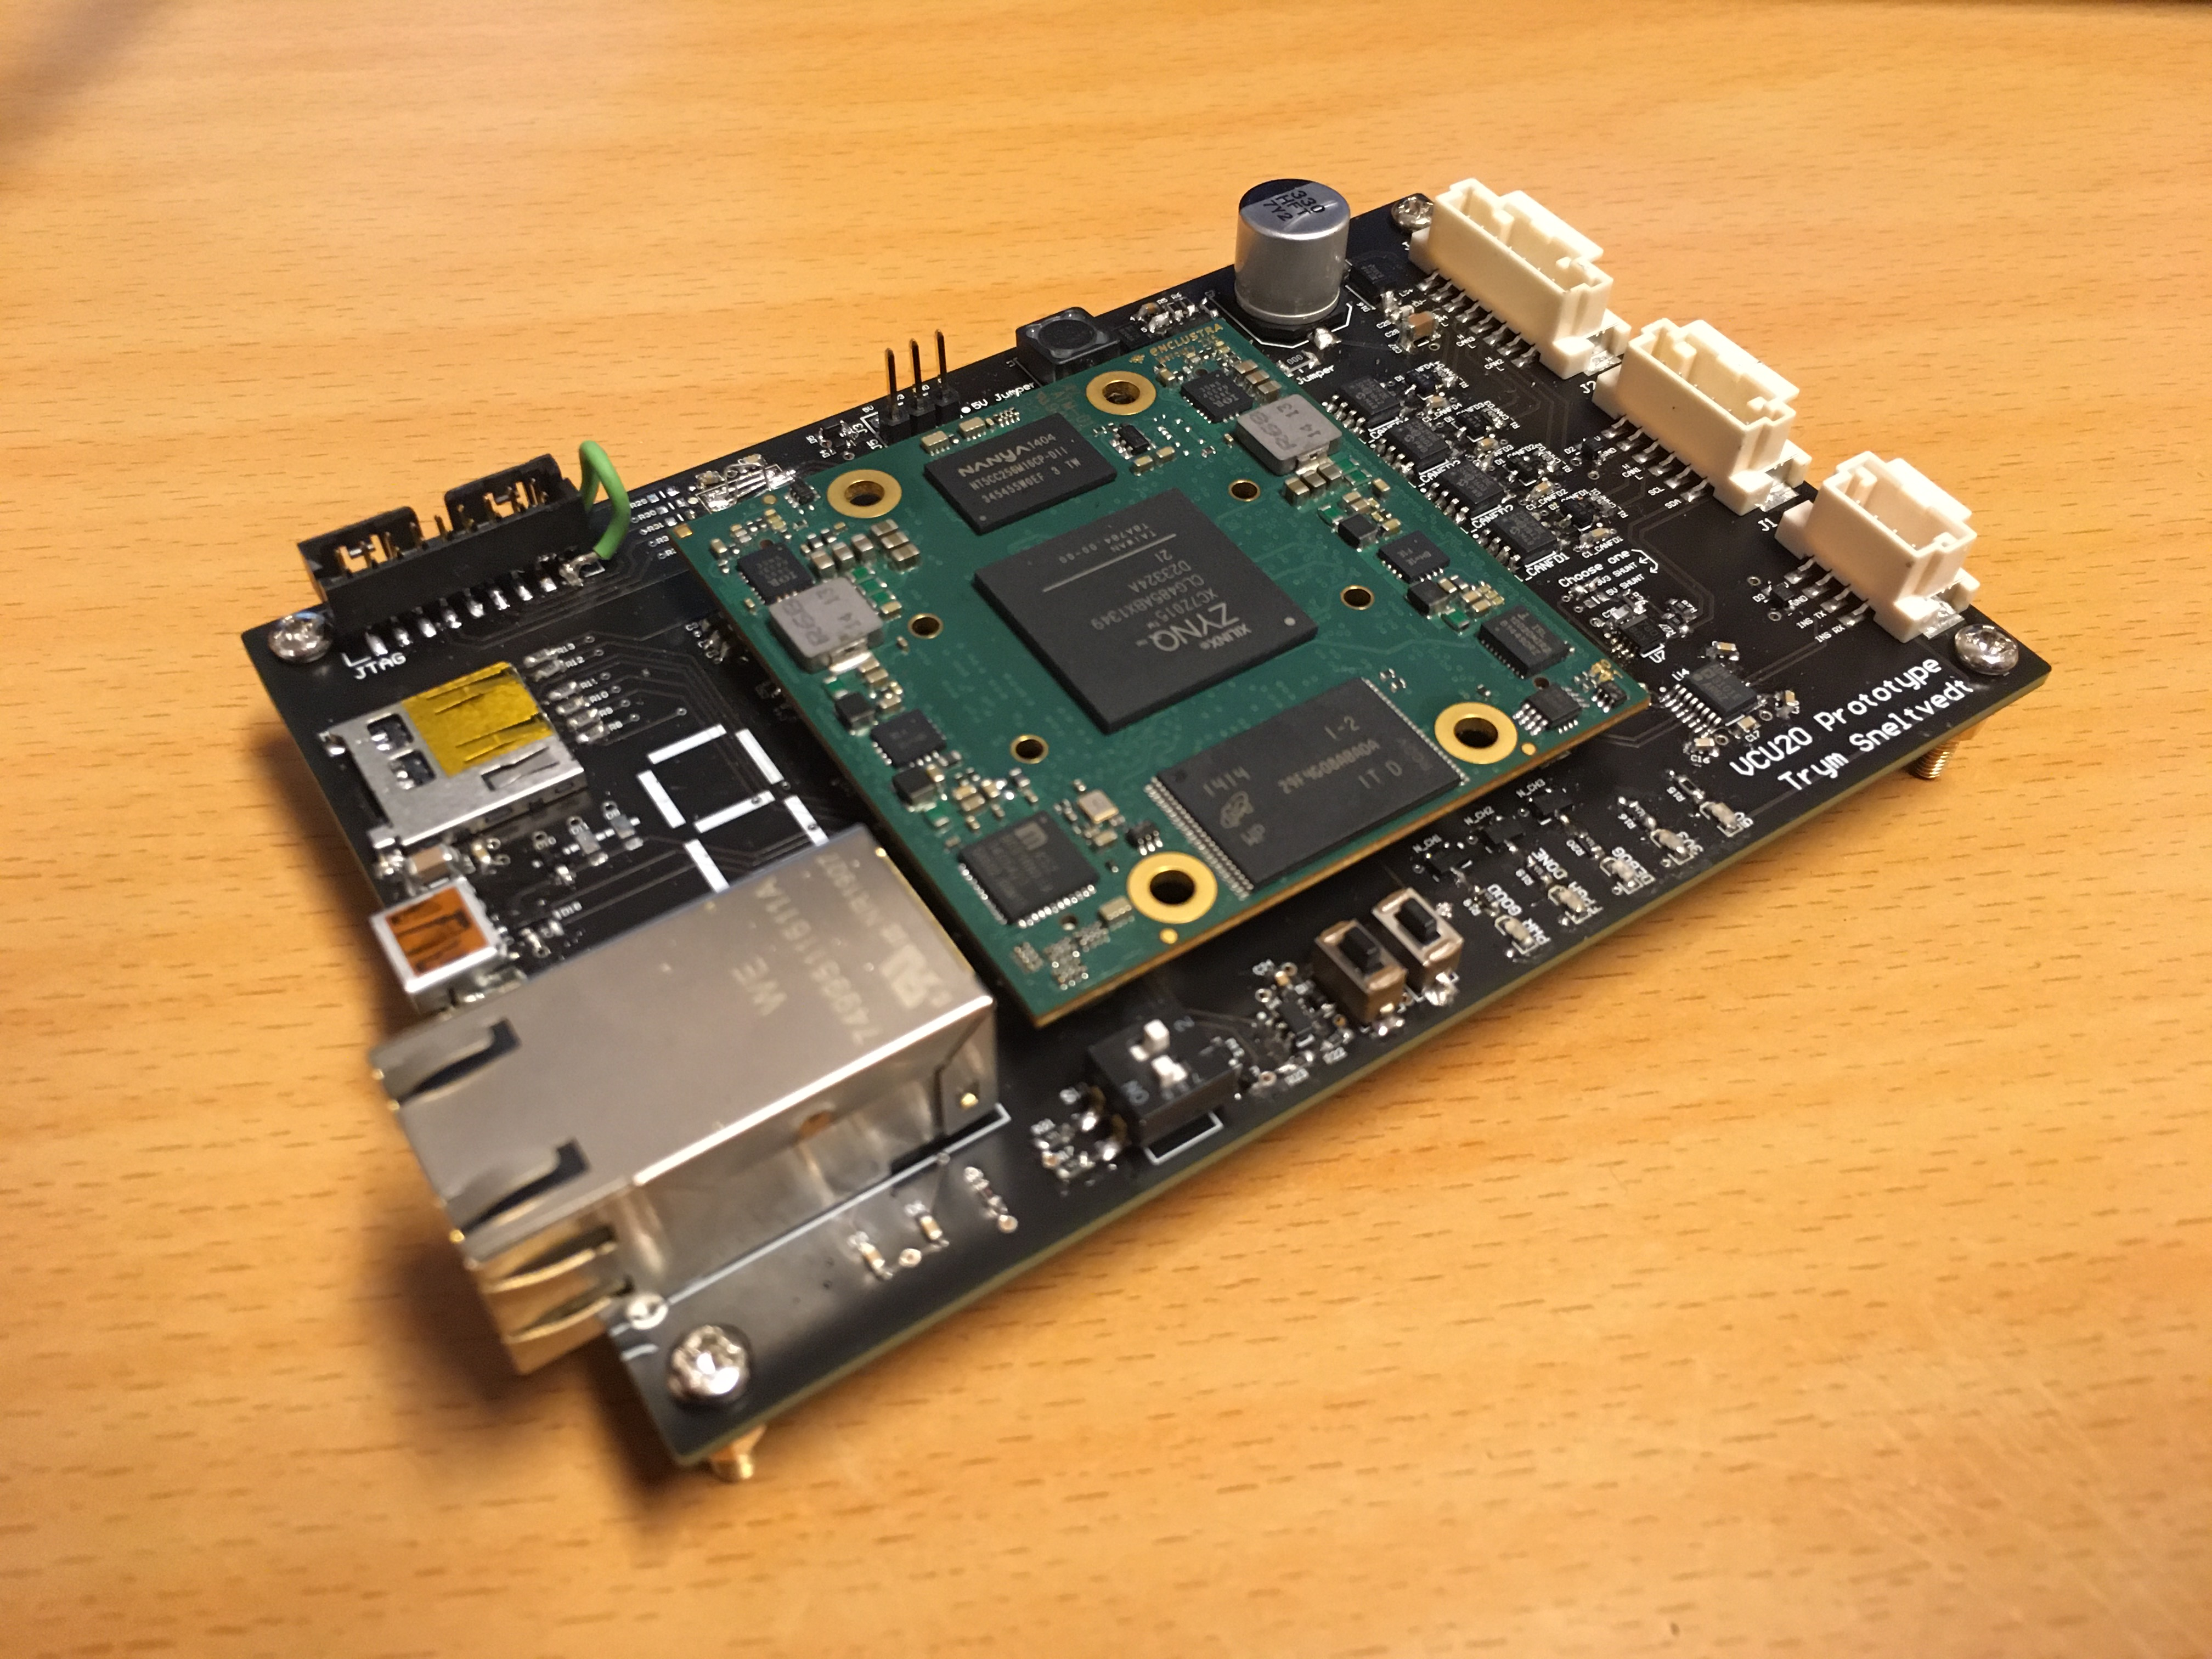
\includegraphics[width=.85\textwidth]{media/vcu20.JPG}
    \caption{VCU20 PCB with all components and Mercury ZX5 module attached}
    \label{fig:vcu20_soldered}
\end{figure}

{\color{red}Must mention CAN-FD interfaces (whether they work or not)}

\subsection{Ethernet bandwidth}

{\color{red} Benchmark Ethernet interface bandwidth. Calculations showing whether it is able to transmit all data from CAN-FD buses over telemetry}

\subsection{Further work}

The proposed solution of an extra CAN-FD bus solely used by the inverters and VCU has room for improvement. CAN-FD buses are designed for communication between several embedded systems. When there are only two embedded systems connected to the bus a point-to-point communication system might be more suitable, like the Ethernet link between the VCU and the telemetry radio. It would be best to utilize one of the unused interfaces on the module as this would reduce the required amount of supporting circuitry. The module is equipped with 4 general purpose Gigabit Transceivers, these would probably be a good fit.

Another solution that the author would recommend to next year's team is to consider merging the VCU and the inverters. The VCU is currently overpowered when considering the relatively simple tasks it performs and it should at least be researched whether the Zynq-7000 could run the inverter control loops in addition to the torque vectoring algorithms. If the ZX5 module proves to be too weak, the team should consider transitioning to the Xilinx Zynq UltraScale+ MPSoC platform. They are equipped with one quad/dual-core ARM Cortex A53 application processors, one dual-core ARM Cortex R5 real-time processor and a FPGA. This should be more than sufficient to run both systems. Possible pitfalls are competition rules, they must be examined closely. The Ultrascale platform is available as modules as well, although at a higher cost compared to the Zynq-7000 series.


